\documentclass[graphic, aspectratio=169]{beamer}

\usepackage{listings}
\usepackage{graphicx}
\usepackage{caption}
\usepackage{subcaption}
\usepackage{hyperref}
\usepackage{tabularx}

\setbeamertemplate{frametitle}[default][center]
\setbeamertemplate{background}
{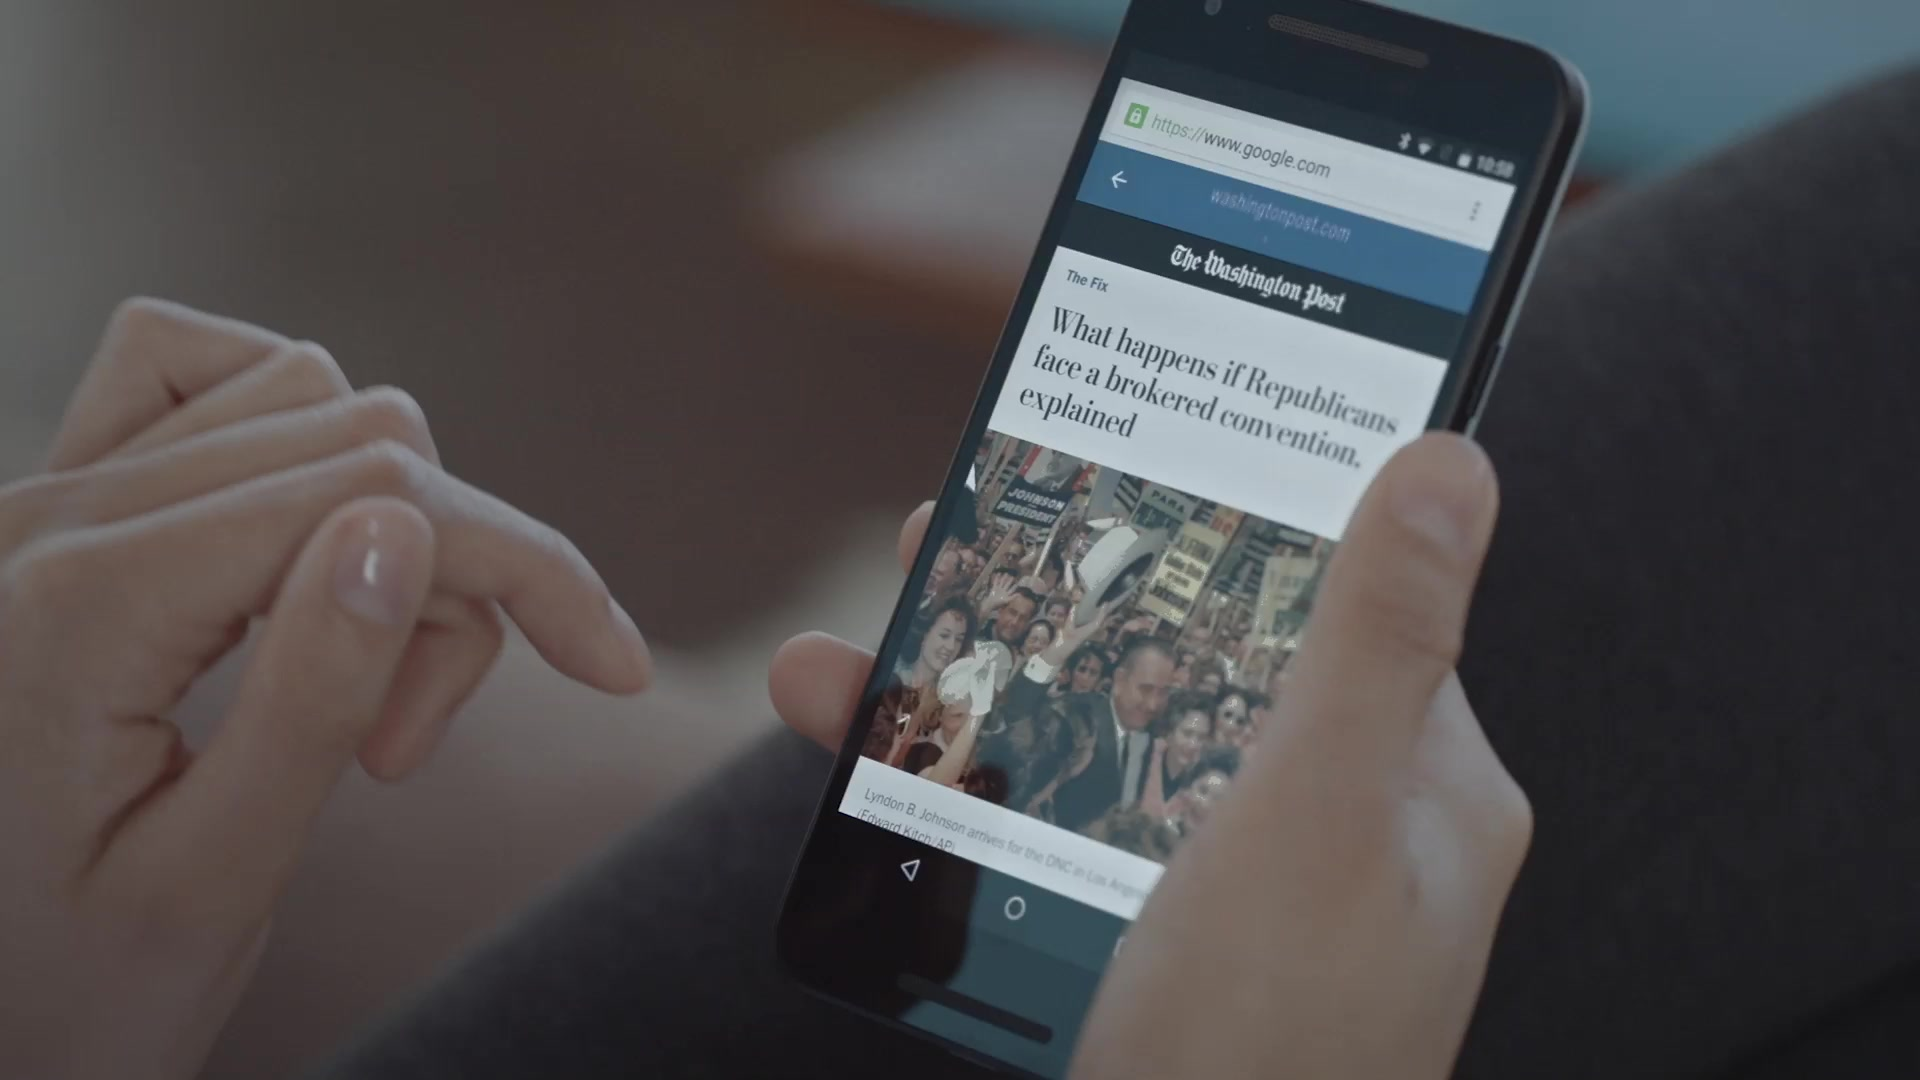
\includegraphics[width=\paperwidth,height=\paperheight,keepaspectratio=true]{images/background.jpg}}

\begin{document}

\begin{frame}
\begin{picture}(300,200)
\put(30,80){
\includegraphics[scale=.1]{images/logo-AMP}}
\put(10,60){
    \textcolor{white}{
        \begin{minipage}[t]{0.4\linewidth}
            {AMP - Accelerated Mobile Pages}
        \end{minipage}
    }
}
\end{picture}
\end{frame}

\setbeamertemplate{background}
{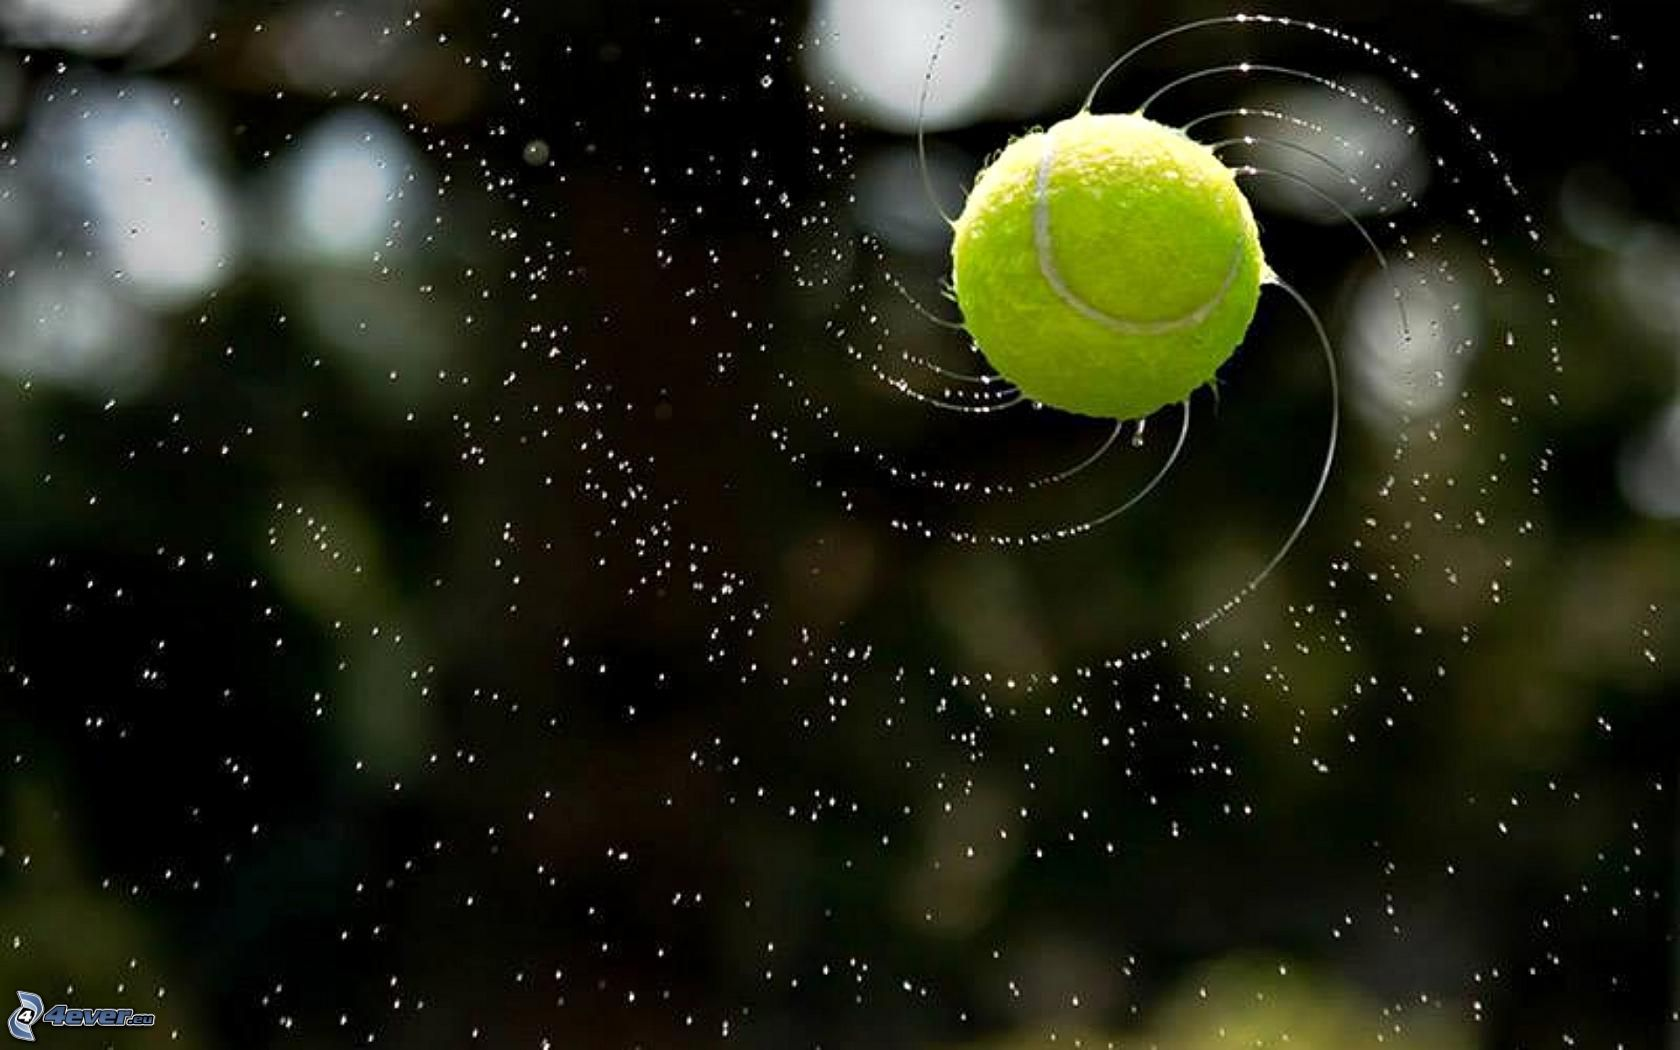
\includegraphics[width=\paperwidth,height=\paperheight]{images/tennis-ball.jpg}}
\begin{frame}
\end{frame}

\setbeamertemplate{background}{} % Imposto il background bianco 
\begin{frame}{}
    \begin{figure}[h!]
    \centering
    
\includegraphics[scale=0.3]{images/google-spdy.jpg}
    \label{fig:Google SPDY}
\end{figure}
    \begin{figure}[h!]
    \centering
    
\includegraphics[scale=0.5]{images/http2.jpeg}
    \label{fig:HTTP/2.0}
\end{figure}

\end{frame}

\begin{frame}
    \begin{figure}
    \centering
        \begin{subfigure}[b]{0.3\textwidth}
        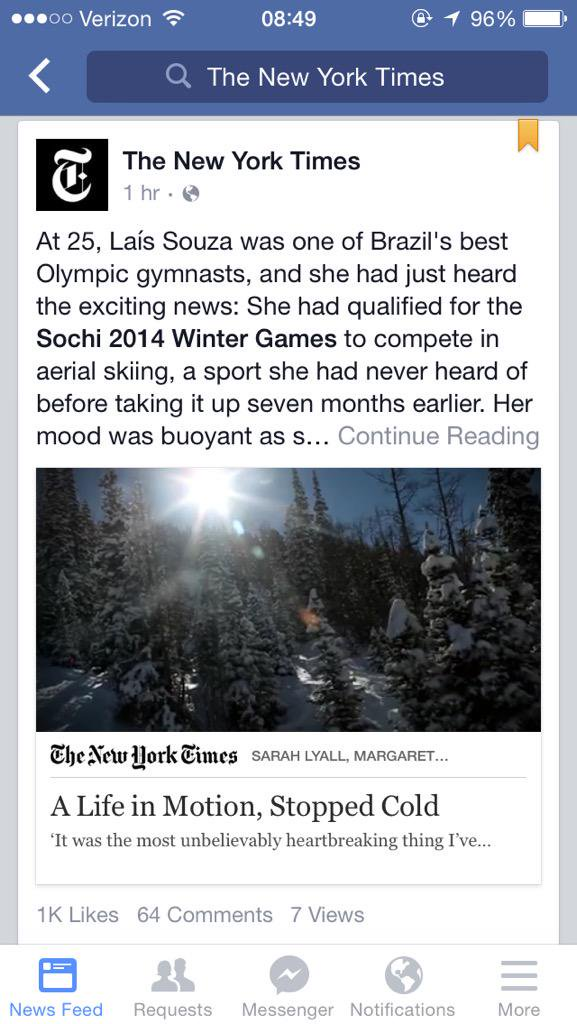
\includegraphics[width=\textwidth]{images/FA_example.jpg}
        \label{fig:Facebook Instant Articles}
    \end{subfigure}
    ~ %add desired spacing between images, e. g. ~, \quad, \qquad, \hfill etc. 
      %(or a blank line to force the subfigure onto a new line)
    \begin{subfigure}[b]{0.4\textwidth}
        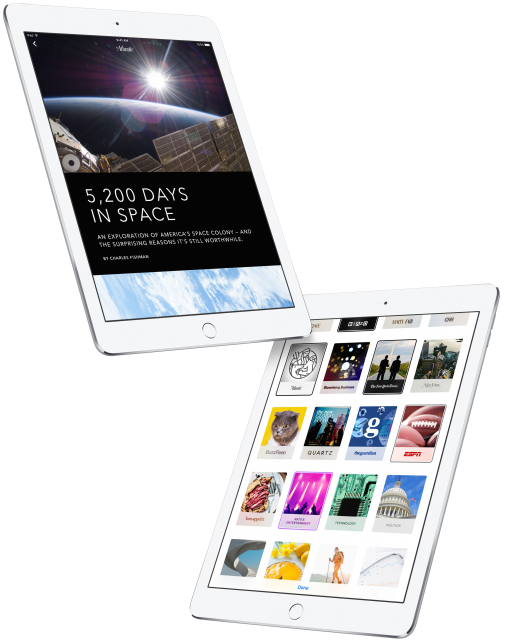
\includegraphics[width=\textwidth]{images/apple_news_format.png}
        \label{fig:Apple News Format}
    \end{subfigure}

    \end{figure}

\end{frame}

\begin{frame}
    \begin{figure}[h!]
    \centering
    
\includegraphics[scale=0.5]{images/FA_supporters.png}
    \label{fig:Facebook Instant Articles}
    \end{figure}
\end{frame}

\setbeamertemplate{background}{} % Imposto il background bianco 

\begin{frame}
    % AMP is a way to build web pages for static content that render fast. AMP in action consists of three different parts:
    % html-amp, AMP js, Google AMP Cache
    \begin{figure}[h!]
    \centering
    
\includegraphics[scale=0.1]{images/logo-AMP.png}
    \label{fig:AMP logo}
    \end{figure}
    \begin{center}
    AMP HTML   -   AMP JS  -  Google AMP Cache
    \end{center}
\end{frame}

\begin{frame}
    % AMP is a way to build web pages for static content that render fast. AMP in action consists of three different parts:
    % html-amp, AMP js, Google AMP Cache
    
\frametitle{AMP HTML}
\lstinputlisting[language=html]{amp-html.html}
\end{frame}

\setbeamertemplate{background}
{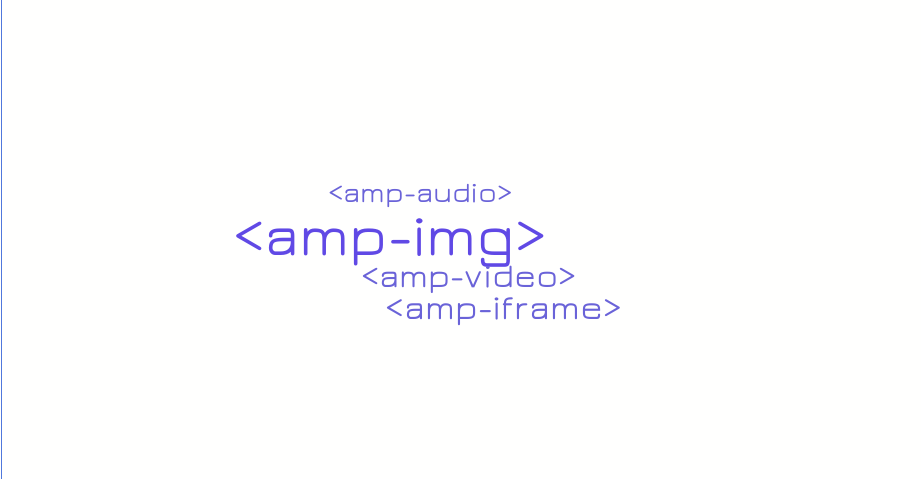
\includegraphics[width=\paperwidth,height=\paperheight]{images/replaced_tags.png}}
\begin{frame}
\end{frame}

\setbeamertemplate{background}
{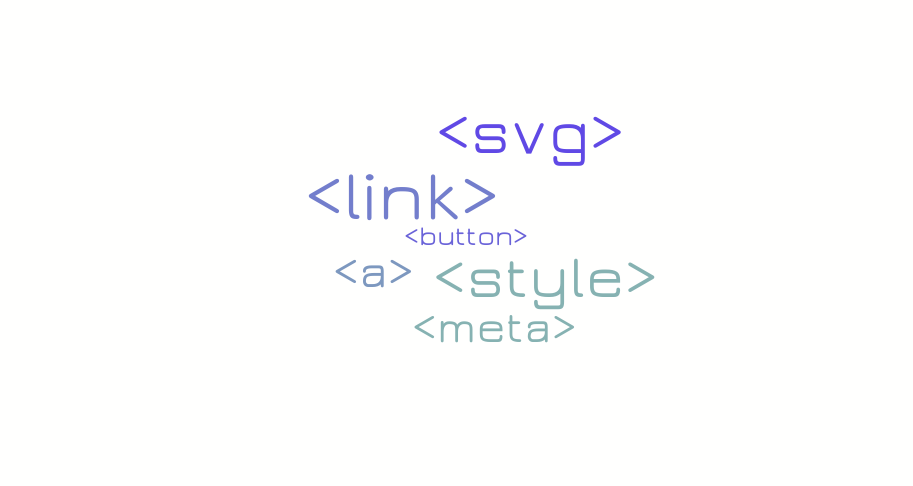
\includegraphics[width=\paperwidth,height=\paperheight]{images/ok_tags.png}}
\begin{frame}
\end{frame}

\setbeamertemplate{background}
{
\includegraphics[width=\paperwidth,height=\paperheight]{images/deprecated_tags.png}}
\begin{frame}
\end{frame}

\setbeamertemplate{background}
{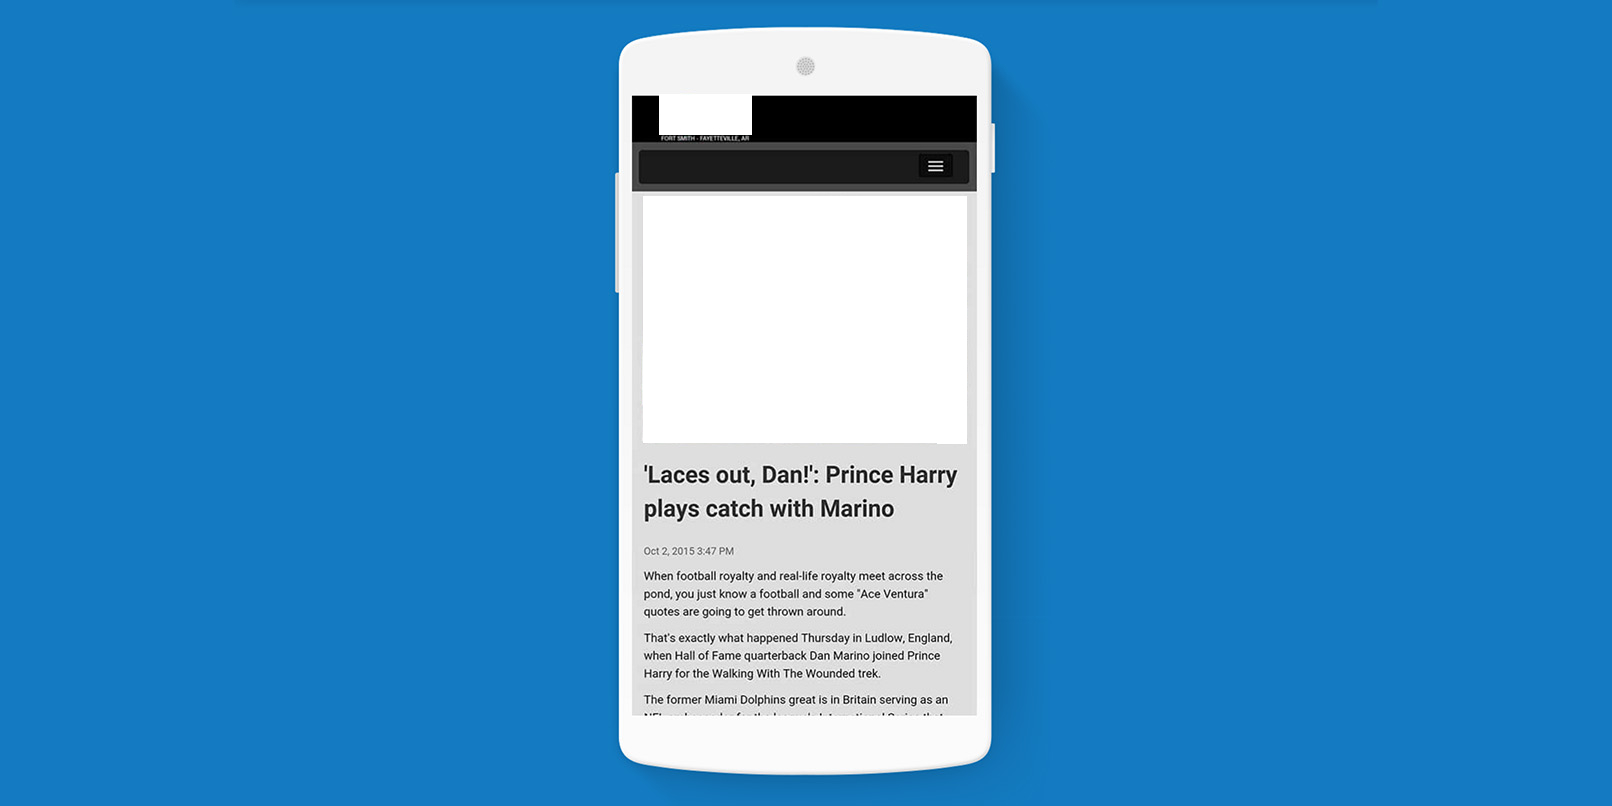
\includegraphics[width=\paperwidth,height=\paperheight]{images/amp_example_without_images.jpg}}
\begin{frame}
\end{frame}

\setbeamertemplate{background}
{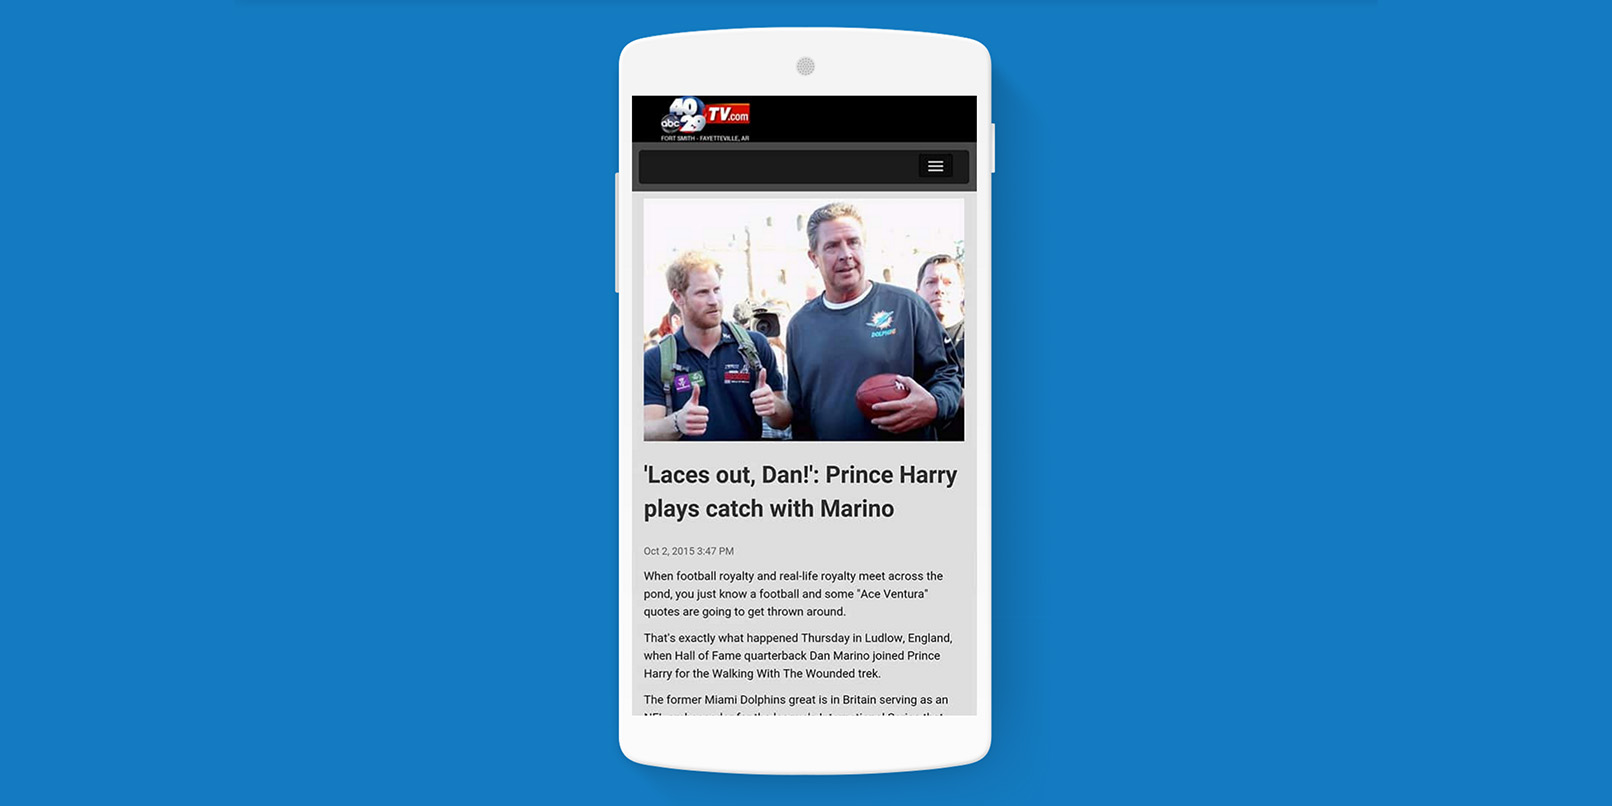
\includegraphics[width=\paperwidth,height=\paperheight]{images/amp_example.jpg}}
\begin{frame}
\end{frame}

\setbeamertemplate{background}
{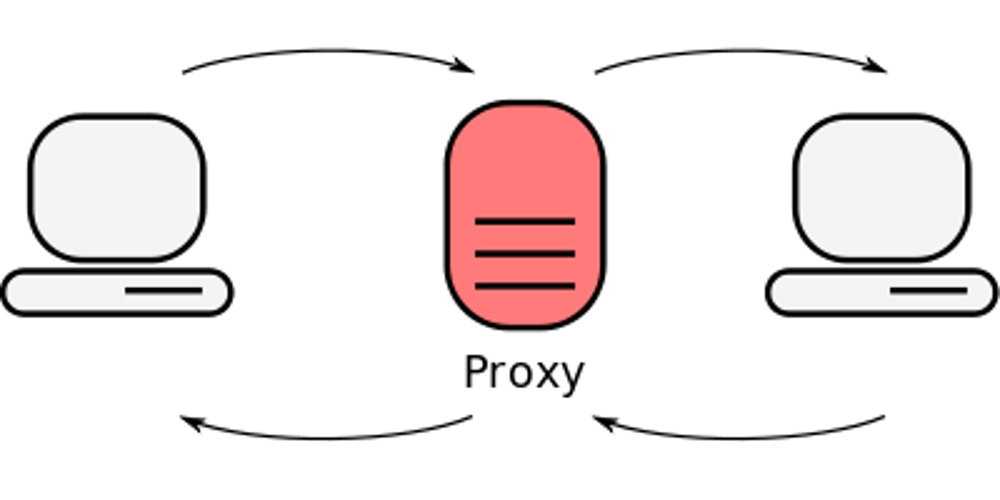
\includegraphics[width=\paperwidth,height=\paperheight]{images/proxy.png}}
\begin{frame}{AMP Cache}
\end{frame}

\setbeamertemplate{background}{} % Imposto il background bianco 
\begin{frame}
    \begin{figure}
        \centering
        
\includegraphics[scale=0.3]{images/amp+wp.png}
        \label{fig:amp+wordpress}
    \end{figure}
    \begin{itemize}
        \item \url{https://wordpress.org/plugins/amp/}
    \end{itemize}
\end{frame}

\begin{frame}

\begin{center}
\begin{tabular}{>{\centering\arraybackslash}p{4cm}}

\includegraphics[height=1cm]{images/twitter_logo.png} \textbf{\href{https://twitter.com/enrico_salvucci}{ @enrico\_salvucci}} \\

\includegraphics[height=1cm]{images/github_logo.png} \textbf{\href{https://github.com/esalvucci}{https://github.com/esalvucci}} \\
\end{tabular}

\bigskip
\begin{footnotesize}
Slides realizzate con \LaTeX\ .\\
La seguente presentazione \`e rilasciata sotto licenza\\
\textbf{\href{http://creativecommons.org/licenses/by-sa/4.0/}{Creative Commons - Attributions, Share-alike 4.0}}\\

\medskip

\includegraphics[height=0.8cm]{images/cc.png}

\medskip
Sorgenti su \textbf{\url{https://github.com/esalvucci/WordpressRomagnaMeetupAMPTalk}}
\end{footnotesize}
\end{center}
\end{frame}

\end{document}
